\documentclass{article}

\usepackage[polish]{babel}
\usepackage[T1]{fontenc}
\usepackage{tabularx}
\usepackage{amsfonts}
\usepackage{amsmath}
\usepackage{mathtools}
\usepackage{enumitem}
\usepackage{graphicx}
\usepackage{algpseudocode}

\begin{document}
    \begin{titlepage}
        \title{Algorymy metaheurystyczne}
        \author{Mateusz Chęciński, Mateusz Tofil}
        \maketitle
    \end{titlepage}

    \section{Wprowadzenie}

    Celem tej listy było zapoznanie się z algorytmami ewolucyjnymi, a w szczególności
    genetycznym (z ang. Genetic Algorithm, GA).

    \section{Opis algortmu}

   Zaimplementowany algorytm jest mocno generyczny, mamy wiele opcji do wyboru.
   Na początku mamy pierwszy etap, tj. generowanie osobnikow.
   Decydujemy, czy podajemy rozwiązania początkowe
   (lub np. funkcję heurystyczną, które takie wygeneruje), czy są
   ono losowe. Są także 2 możliwe warunki zakończenie:
   liczba pokoleń lub czas.
   Następnie przebieg algorytmu opiera się na selekcji, krzyżowaniu i
   ewentualnej mutacji.
   Zaimplementowaliśmy 3 opcje wyboru:
   1) Losowy – każdy osobnik ma równe szansa bycia wybranym
   2) Ruletka – lepiej przystosowane osobniki mają większą szanse bycia wybranym niż słabsze
   (losowanie z różnymi prawdopodobieństwami)
   3) Turniej – wybór najlepszego osobnika z pośród k losowych osobników
   Wybieramy połowę z osobników na rodziców (osobnik lepiej przystosowany
   może się powtorzyć), ponieważ każda para ma dwójkę dzieci, a chcemy
   zachować rozmiar populacji.
   Korzystamy z trzech dostępnych operatorów krzyżowania: HX, OX, PMX.
   Następnie zgodnie z podanym przez użytkownika prawdopodobieństwem
   i zadaną funkcją (invert, insert, swap) zachodzi losowa mutacja.
   Po wszystkich iteracjach zwracany jest najlepszy osobnik.

    \noindent Język programowania: Python 3.10

     \section{Porównanie selekcji: losowe, ruletka, turniej}

    W celu zbadania jaka selekcja jest najlepsza z
    powyższych 3, przeprowadziliśmy eksperymenty wywołując
    metode ze zmienionym parametrem początkowym. Wszystkie
    eksperymetry były przeprowadzone dla tej samej instacji
    wraz z tym samym rozwiązaniem początkowym. Wykres poniżej
    został wykonany dla intacji o macierzy pełnej.

    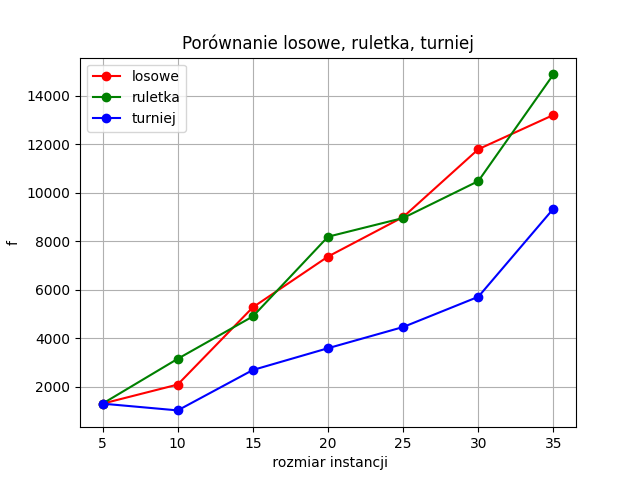
\includegraphics[width=11cm]{./spr3img/Figure_1FULL.png}

    Następnie przeprowadziliśmy ten sam eksperyment, z tą różnicą
    że teraz dla przestrzeni euklidesowej.

   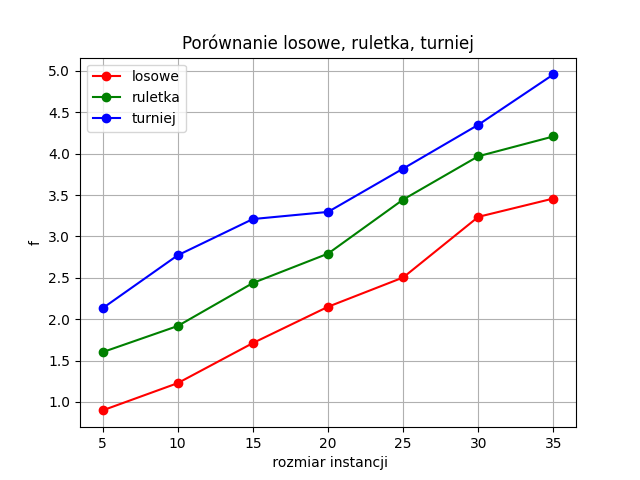
\includegraphics[width=11cm]{./spr3img/Figure_2.png}

    Jak możemy zauważyć, dla wszystkich przeprowadzonych
    przez nas intacji, selekcja \emph{losowa} okazała się być
    najelpszym. Pozostałe selekcje też nie są źle. Wszystkie
    selekcje działają w czasie $\mathcal{O}(n)$ i różnią się tylko
    stałą, najmniejszą stałą posiada \emph{losowa}. Wynika to z faktu,
    że w pozostałych do losowania dodajemy jeszcze pewne założenia.

    Poprzednio porównaliśmy jak czas działa dla poszczegołnych selekcji. Teraz
    porównamy jak wybór selekcji wpływa na koszt cyklu dla tych samych
    intacji. Ponwnie wykresy, przzygotowaliśmy dla instacji pełnej ograniczeniami
    dla przestrzeni euklidesowej. Wykresy w odpowieniej kolejności zostały
    wstawione poniżej.

    Dla instacji o macierzy pełnej, wygenerowanej losowo.

    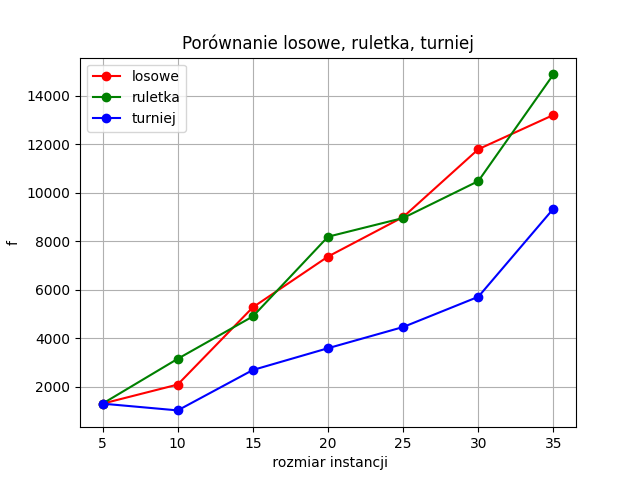
\includegraphics[width=11cm]{./spr3img/Figure_1FULL.png}

    Dla instacji z macierzą, wypełnioną odległościami z przestrzeni
    euklidesowej.

    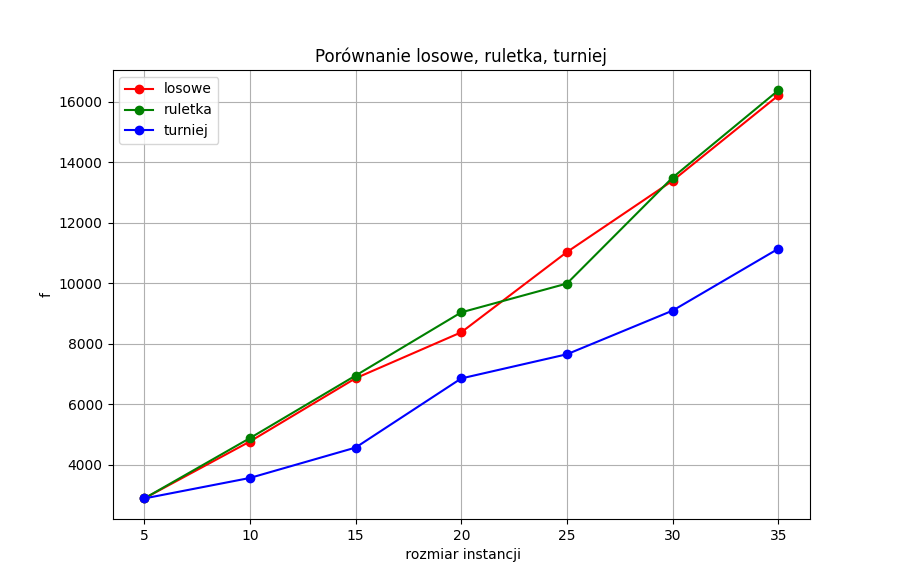
\includegraphics[width=11cm]{./spr3img/Figure_1.png}

    Tym razem \emph{losowa} nie był najlepszym wyborem z możliwych przez nas
    zaimplementowanych otoczeń. Teraz najlepszy okazał się \emph{turniej}.
    Wybierając właśnie ten sposób selekcji dla przebadanych instacji, mogliśmy się
    spodziewać funkcji kosztu o najniższej wartośći. Jednocześnie należy zauwważyć,
    że zajmuje ono najdłuższy czas.

    \section{Porównanie krzyżowań: HX, OX, PMX}

     W celu zbadania jakie krzyżowanie jest najlepsze z
    powyższych 3, przeprowadziliśmy analogiczne eksperymenty.
    Najpierw czas.

     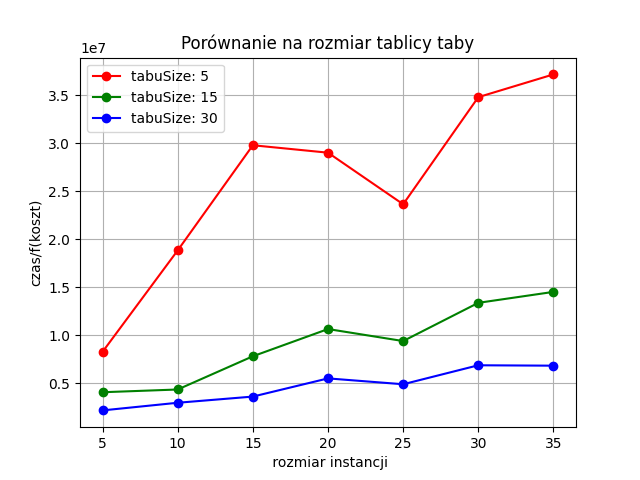
\includegraphics[width=11cm]{./spr3img/Figure_4.png}

    Dla przestrzeni euklidesowej

    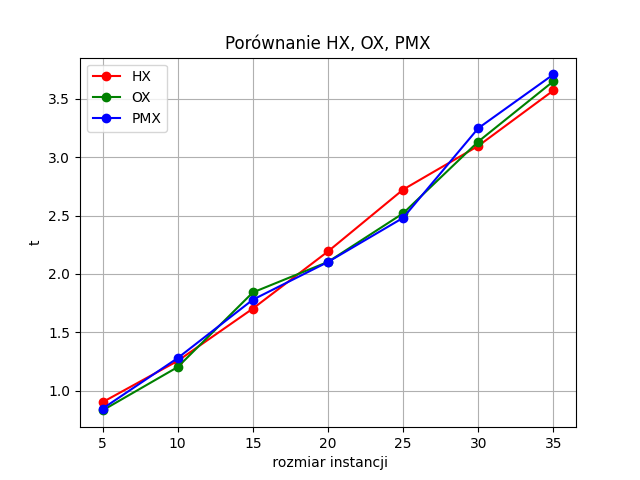
\includegraphics[width=11cm]{./spr3img/Figure_4EUC.png}

    Teraz wartość funkcji celu.

    Dla instacji o macierzy pełnej, wygenerowanej losowo.

    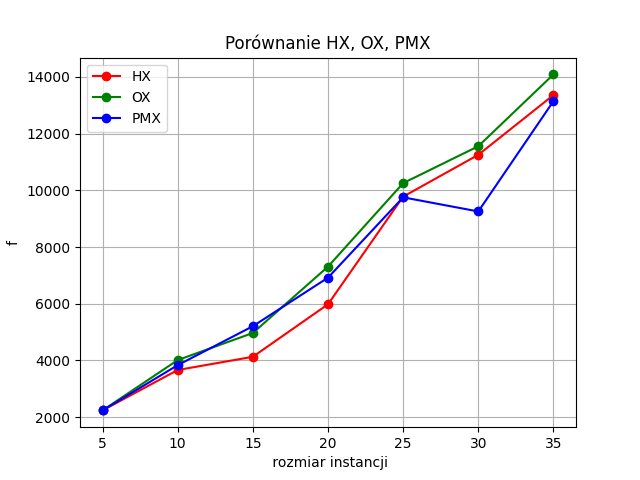
\includegraphics[width=11cm]{./spr3img/Figure_3FULL.png}

    Dla instacji z macierzą, wypełnioną odległościami z przestrzeni
    euklidesowej.

    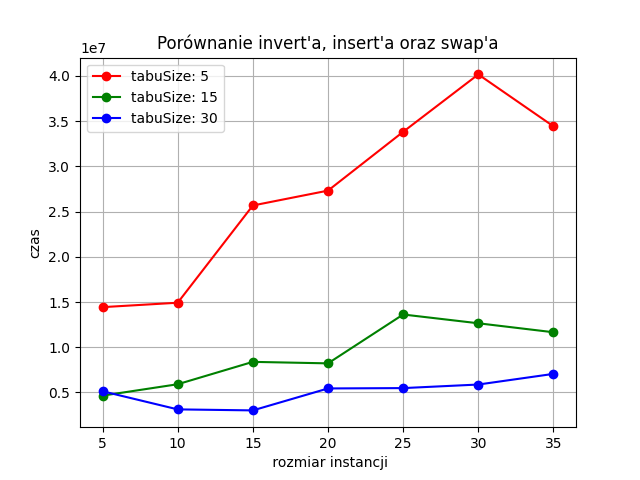
\includegraphics[width=11cm]{./spr3img/Figure_3.png}

   Jak widać żadne z krzyżowań się nie wyróżniło. Wszystkie mają podobny
   czas i efektywność, wykresy wzajemnie się przecinają w zależności od
   instancji.

    \section{Porównanie prawdopodobieństwa mutacji}

    Najpierw zbadaliśmy wpływ częstości mutacji na czas

    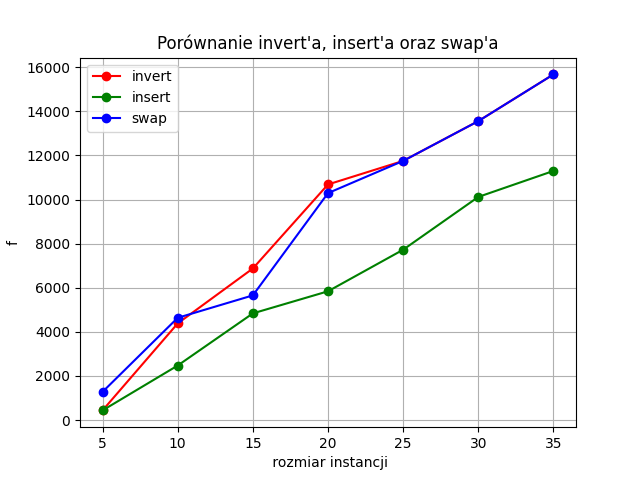
\includegraphics[width=11cm]{./spr3img/Figure_5.png}

    Jak widać im częsciej robimy mutacje, tym dłużej działa algorytm.

    Ważniejszy jest jednak wpływ prawdopodobieństwa mutcji na końcowy wynik.

     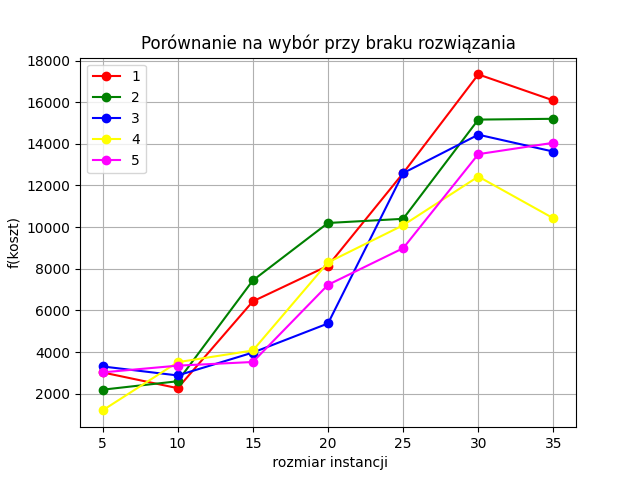
\includegraphics[width=11cm]{./spr3img/Figure_6.png}

     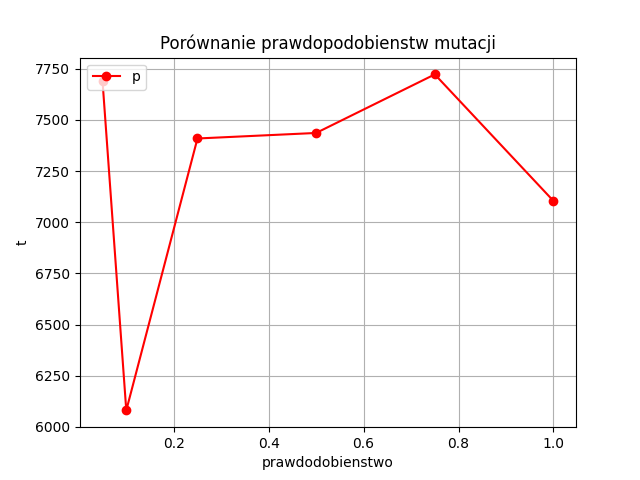
\includegraphics[width=11cm]{./spr3img/Figure_62.png}

     Można zauważyć, że nie ma szczególnej zasady, co do wpływu częstości
     mutacji na wynik. Analizując jednak oba te wykresy oraz wykres czasu
     najkorzystniejszy jest wybór w okolicach 5%.

    \section{Warunek stopu}

    TODO: zostawiamy to samo? XDD

    Zaimplemnetowaliśmy trzy różne warianty zatrzymanai się algorytmu.
    Pierwszy z nich zaznaczono na czerwono na poniższym wykrysie jest ilość ogólnej
    iteracji algoyrtmu. Drugi z koleji, na zielono, ilość iteracji algorytmu, gdzie
    nie znaleźliśmy lepszego rozwiązania, przez k-iteracji. Ostatnim z koleji jest, czas,
    zaznaczony kolorem niebieskim.

    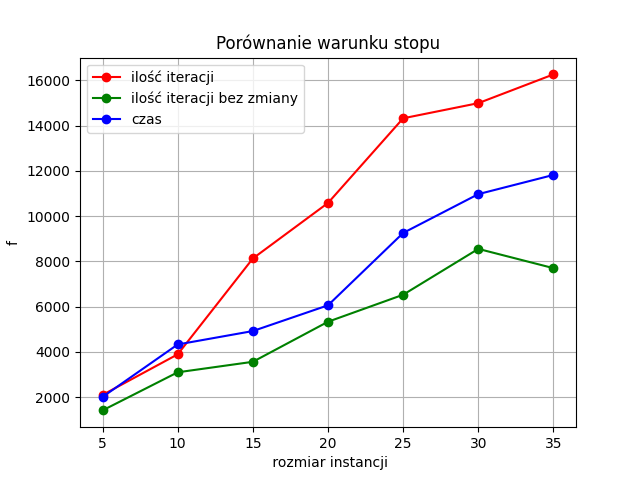
\includegraphics[width=11cm]{./spr2img/Figure_8.png}

    Funckja kosztu dla ogarniczenia samymi iteracjami jest znacząco większa niż liczenie
    iteracji bez zmian. Jest to naturalne zachowanie, wynikające z faktu, że prawie zawsze

    $$I + K = iteracje(iloscBezZmian) > iteracje(zwykle) = I$$

    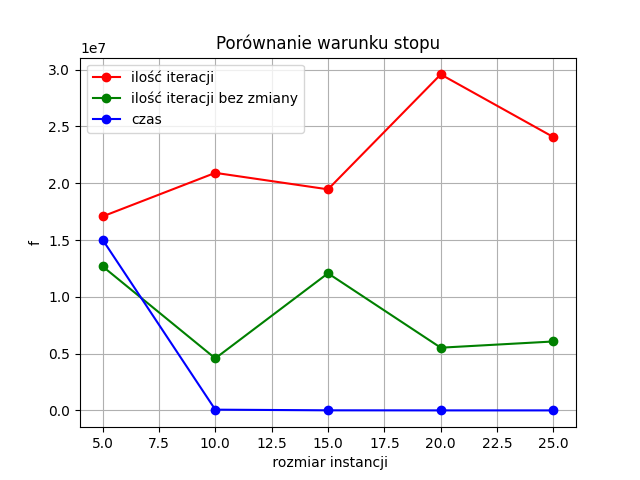
\includegraphics[width=11cm]{./spr2img/Figure_10.png}

    Jak można było się spodziewać, ilość iteracji bez zmiany zdecydowanie korzystniej
    wpływa na funckje kosztu niż sama ilość iteracacji. Teraz porównamy, jak
    warunek stopu wpływa na efektywność optymalnego rozwiązania. Jeżeli wybierzemy odpowiednio duży czas,
    to algorytm będzie tak długo pracował, aż zdajdzie optymalne rozwiązanie. Inaczej jest trochę
    z ograniczeniami na ilośc iteracji. Można było się spodziewać, że w wariancie, gdzie liczby iteracje
    bez zmian, współczynniki  efektywności będzie znacznie lepszy od samego liczenia iteracji.
    Jest to oczywiste, bo iteracje wykonujemy za każdym razem, a iteracji bez zmian wykonamy dodatkowo więcej,
    na koniec działania algorytmu, niż samo liczenie iteracji.

    \section{Złożoność obliczeniowa algortmu genetycznego}

    Złożonośc obliczeniowa zależy od wielu czynników takich jak:
    rozmiar populacji, typ selekcji, czy krzyżowania.

    TODO

    \section{Algorytm genetyczny dla gr120}

    TODO



\end{document}